\section{Memorandum}
\noindent\textbf{Date:} February 9, 2021\\
\textbf{To:} the Washington State Department of Agriculture\\
\textbf{From:} MCM Team 2100585\\
\textbf{Subject:} Identifying the sighting reports of Vespa mandarinia\\
\rule[-7pt]{14.3cm}{0.1em}

\noindent Dear Sir or Madame,

In accordance to your requests, we establish a system for prioritizing sighting reports and we also analyze relevant information about pest through data analysis. 
    Then we are writing to report our key results in these four days.

\centerline{\bf Prioritization System}
We will introduce the priority ranking system we designed from the order of the data processing flow.
\begin{enumerate}[\quad\bf Step1.]
    \item \textbf{Image Recognition.} We use the ready-made insect recognition platform with high accuracy to recognize the pictures in the report, and the output result is the name of a certain insect or it cannot be recognized. If the result is the latter then it will be put in screen-out zone. If it is the former then save the insect name.
    \item \textbf{Text processing.} We use logistic regression to measure the validity of the text in the report, and finally output a score. 
    \item \textbf{Data Screening.} If the score of a report in the screen-zone is lower than the threshold we set, the report will be discarded.
    \item \textbf{Run PS-CA model.} Based on the CA model, we simulate the regional distribution of pests over time. And then get the probability of pests appearing in the area under the detection time.
    \item \textbf{Get scores for four indices.} The first indicator is the probability of pest appearing here ,which has been obtained in Step4. The second one is the activeness of the pest at this time, which can be obtained by the pest’s habits. The third one is the information of note, which has been obtained by Step2. The fourth one is the similarity between the insects identified by the image and the pest, which can be obtained in the FCEM-AHP model according to the names of the insects.
    \item \textbf{Sorting based on TOPSIS.} In the last step, we only need to use TOPSIS to rank each report according to the scores of the four indicators.
\end{enumerate}

\centerline{\bf Conclusions}

In order to better present our conclusions, we visualize all the results and present them below.

\begin{figure}[H]
    \centering
    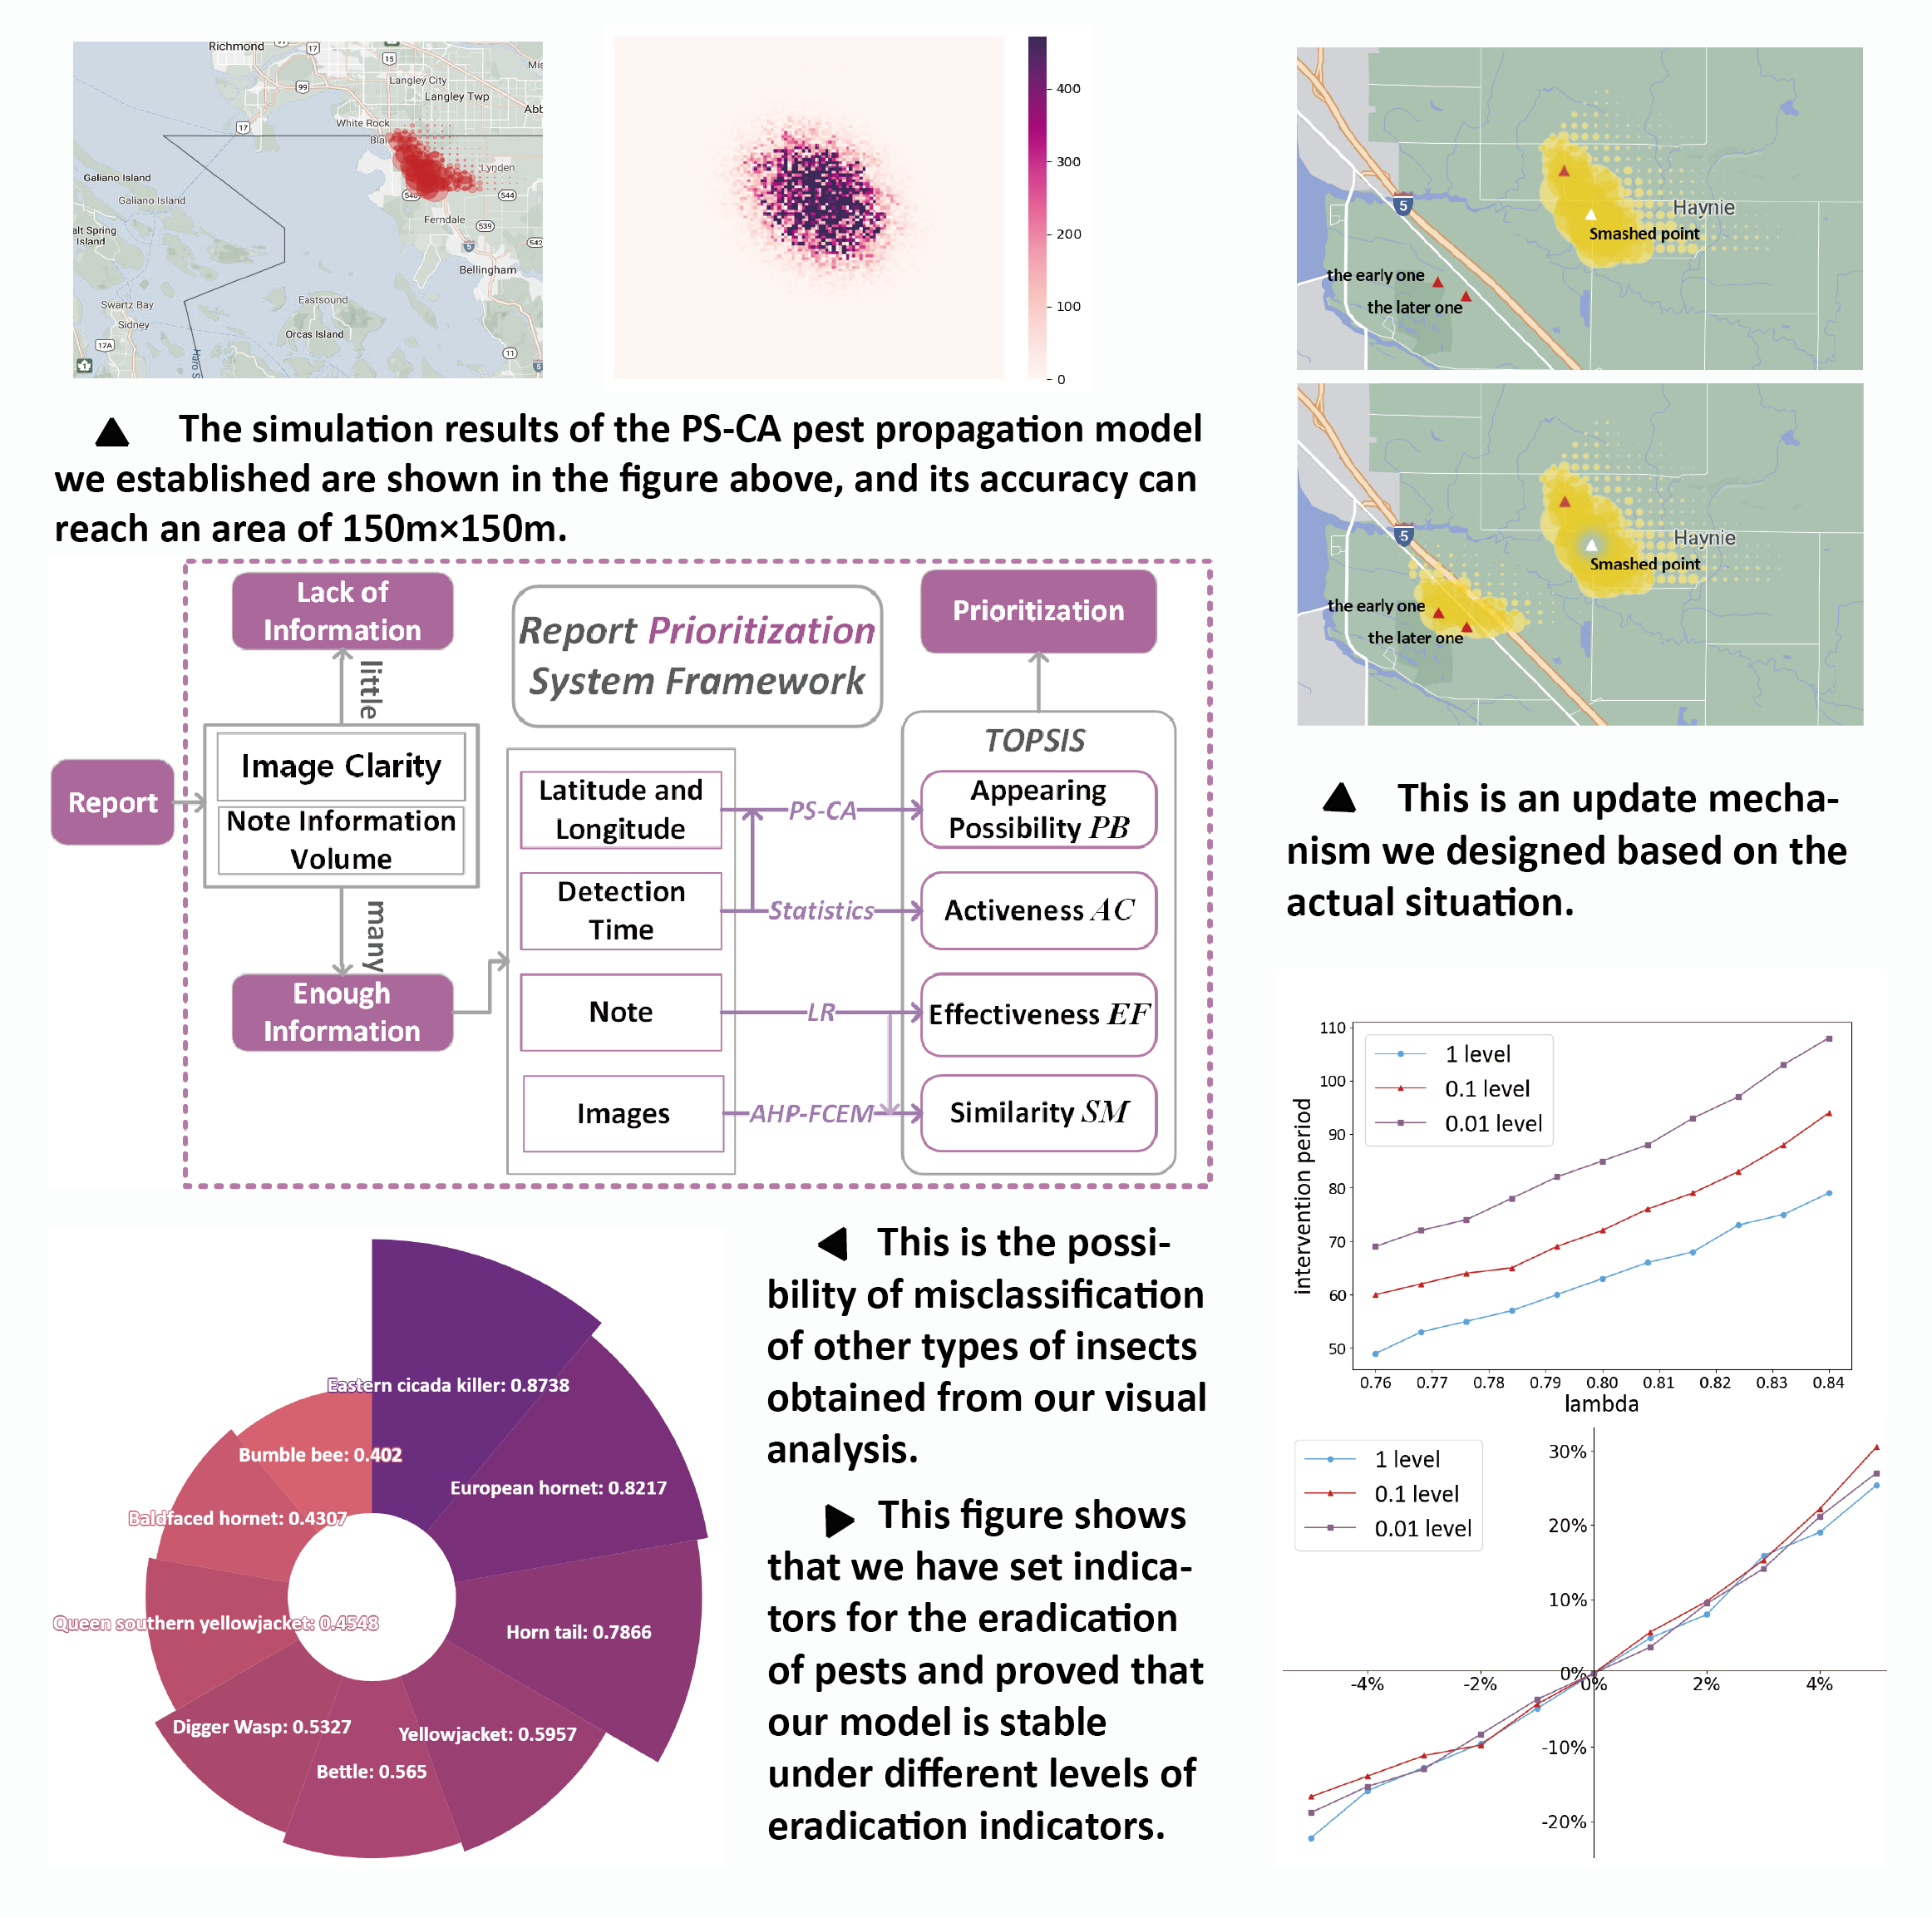
\includegraphics[scale = 0.7]{Chapter-2021C/images-2021C/post.png}
    % \caption{Emerging Possibility of the Pest after one year simulation.}
    % \label{fig:2021C-relitu}
\end{figure}
\vspace{-0.5cm}
\begin{enumerate}[\quad\bf1.]
    \item Our team established a model called \textbf{PS-CA }. This simulation is based on Washington's vegetation coverage and cellular automata model. The simulation results are shown in this paper. Moreover, its accuracy can achieve the precision of a $150m \times 150m$ area.%记得写预测结果和精度
    \item The \textbf{FCEM-AHP model} is applied to evaluate likelihood of mistaken classification from a visual perspective. In this article, we present the result of the similarity of nine types of insects of pest. 
    \item \textbf{Prioritizing sighting reports} is our ultimate goal. Its process steps have been clearly shown above. The TOPSIS method and comprehensive indices ensure the rationality of our prioritization. %记得写这个系统的优越性
    \item \textbf{Determining the update mechanism of our prioritization system }is a big step for us to optimize the model. We design a detailed update rule including the frequency that maintains the simulation accuracy. %记得略写更新机制和频率
    \item Our team offers \textbf{evidence of pest eradication} and conducts sensitivity analysis. We define an index and set three criteria to imply the degree of eradication.%记得描述指标
    
    % \textbf{Estimating the possibility of other types of insects being mistaken for Asian bumblebees} is also extremely important and will produce significant results. We are proud that we achieved this task and obtained gratifying data results. We interpret the possibility of being misclassified as the similarity between the type of insect and the pest under study, which can be derived from the comparison of characteristics between the two insects.  We select nine other types of insects for similarity comparison to obtain data on the likelihood of their being misclassified, as shown in Figure \ref{}.
    % \item \textbf{Prioritizing sighting reports} is our ultimate goal. We believe that the method to distinguish between valid reports and invalid reports is to measure the amount of information reported by \textbf{calculating image clarity and related word frequency}. Secondly, the indicators to identify the accuracy of the report should include \textbf{the possibility of appearing here, the possibility of appearing at this time, the amount of information contained in note, and the most important index——the result of image recognition}. The calculation method of these indicators is basing on the existing SP-CA, FCEM-AHP and LR model. After obtaining these four indicators, we can use \text{TOPSIS} to score each report, and finally prioritize it according to the evaluation scores.
    % \item \textbf{Our ranking results are consistent with reality.}
    % In order to test the accuracy of our prioritization system, we randomly sampled several sets of data to rank them and achieved positive results.
    % \item \textbf{Determining the update mechanism of our prioritization system }is a big step for us to optimize the model. Since pest will invade from time to time, we have to \textbf{update our PS-CA model when a new invasion point is discovered}.A new intrusion point will be used as the starting point and simulate together with the original starting point until all pest sighting points are covered. In addition, our model needs to \textbf{adjust the pest growth curve every year} because environmental capacity and human intervention will also affect the pest transmission rate.
    % \item Our team offers provides \textbf{evidence of pest eradication} and conducts sensitivity analysis.
\end{enumerate}

In a nutshell, our results show that \textbf{human intervention is necessary} to prevent the pest spread and \textbf{more efforts and resources} are needed for a thorough eradication.
